\documentclass[12pt]{article}
\usepackage[margin=2.5cm]{geometry}

\usepackage[english]{babel}
\usepackage[utf8]{inputenc}
\usepackage[T1]{fontenc}
\usepackage{amsmath}
\usepackage{esint}
\usepackage{amssymb}
\usepackage{csquotes}
\usepackage{mathtools, graphicx, hyperref, url, svg}
\usepackage{caption}
\usepackage{subcaption}
\usepackage{systeme}
\usepackage{esvect}
\usepackage{amsmath,systeme}
\usepackage{multirow}
\makeatletter
\renewcommand*\env@matrix[1][*\c@MaxMatrixCols c]{%
  \hskip -\arraycolsep
  \let\@ifnextchar\new@ifnextchar
  \array{#1}}
\makeatother

\usepackage{biblatex} %Imports biblatex package
\addbibresource{references.bib}


% För att färga tabellkoloumner
\usepackage{colortbl}

\newcommand{\mc}[2]{\multicolumn{#1}{c}{#2}}
\definecolor{LightCyan}{rgb}{0.88,1,1}

%\newcolumntype{a}{>{\columncolor{Gray}}c}
%\newcolumntype{b}{>{\columncolor{white}}c}

%% För att skriva koden
\usepackage{listings}
\usepackage{color}
\usepackage{inconsolata}

\definecolor{codegreen}{rgb}{0,0.6,0}
\definecolor{codegray}{rgb}{0.5,0.5,0.5}
\definecolor{codepurple}{rgb}{0.58,0,0.82}
\definecolor{backcolour}{rgb}{0.95,0.95,0.92}


\lstset{frame=tb,
  language=Python,
  aboveskip=3mm,
  belowskip=3mm,
  showstringspaces=false,
  columns=flexible,
  basicstyle={\small\ttfamily},
  numbers=none,
  backgroundcolor=\color{backcolour},
  numberstyle=\tiny\color{codegray},
  keywordstyle=\color{magenta},
  commentstyle=\color{codegreen},
  stringstyle=\color{codepurple},
  breaklines=true,
  breakatwhitespace=true,
  tabsize=3
}

\lstset{literate=
  {á}{{\'a}}1 {é}{{\'e}}1 {í}{{\'i}}1 {ó}{{\'o}}1 {ú}{{\'u}}1
  {Á}{{\'A}}1 {É}{{\'E}}1 {Í}{{\'I}}1 {Ó}{{\'O}}1 {Ú}{{\'U}}1
  {à}{{\`a}}1 {è}{{\`e}}1 {ì}{{\`i}}1 {ò}{{\`o}}1 {ù}{{\`u}}1
  {À}{{\`A}}1 {È}{{\'E}}1 {Ì}{{\`I}}1 {Ò}{{\`O}}1 {Ù}{{\`U}}1
  {ä}{{\"a}}1 {ë}{{\"e}}1 {ï}{{\"i}}1 {ö}{{\"o}}1 {ü}{{\"u}}1
  {Ä}{{\"A}}1 {Ë}{{\"E}}1 {Ï}{{\"I}}1 {Ö}{{\"O}}1 {Ü}{{\"U}}1
  {â}{{\^a}}1 {ê}{{\^e}}1 {î}{{\^i}}1 {ô}{{\^o}}1 {û}{{\^u}}1
  {Â}{{\^A}}1 {Ê}{{\^E}}1 {Î}{{\^I}}1 {Ô}{{\^O}}1 {Û}{{\^U}}1
  {œ}{{\oe}}1 {Œ}{{\OE}}1 {æ}{{\ae}}1 {Æ}{{\AE}}1 {ß}{{\ss}}1
  {ç}{{\c c}}1 {Ç}{{\c C}}1 {ø}{{\o}}1 {å}{{\r a}}1 {Å}{{\r A}}1
  {€}{{\EUR}}1 {£}{{\pounds}}1
}

\setlength{\parskip}{1em} % Lämna en blankrad
\setlength{\parindent}{0em} % Indentera inte nya stycken

%%% TITEL %%%

\title{Exercise 4  - Classification}
\author{\textit{Computer Assisted Image Analysis 1  - 1TD396}  \vspace{1cm} \\
         Jennifer Andersson, David Björk \& Tove Gunnarsson \vspace{0.7cm}\\
        }
\date{\today}

%%% DOKUMENTET %%%
\begin{document}
\maketitle

\begin{figure}[b]
  \centering
  \includegraphics[width = 3cm]{images/UU_logo.pdf}
\end{figure}
\thispagestyle{empty}

\clearpage
%\tableofcontents

\newpage
%%%%%%%%%%%%%%%%%%%%%%%%% INTRODUCTION %%%%%%%%%%%%%%%%%%%%%%%%%%%%%%
\section{Classification Basics}


\textbf{\emph{Question 1.}}
% Are the two classes possible to separate by using either the x or y coordinate as a single feature? 
% Explain why or why not.

\begin{figure}[b]
  \centering
  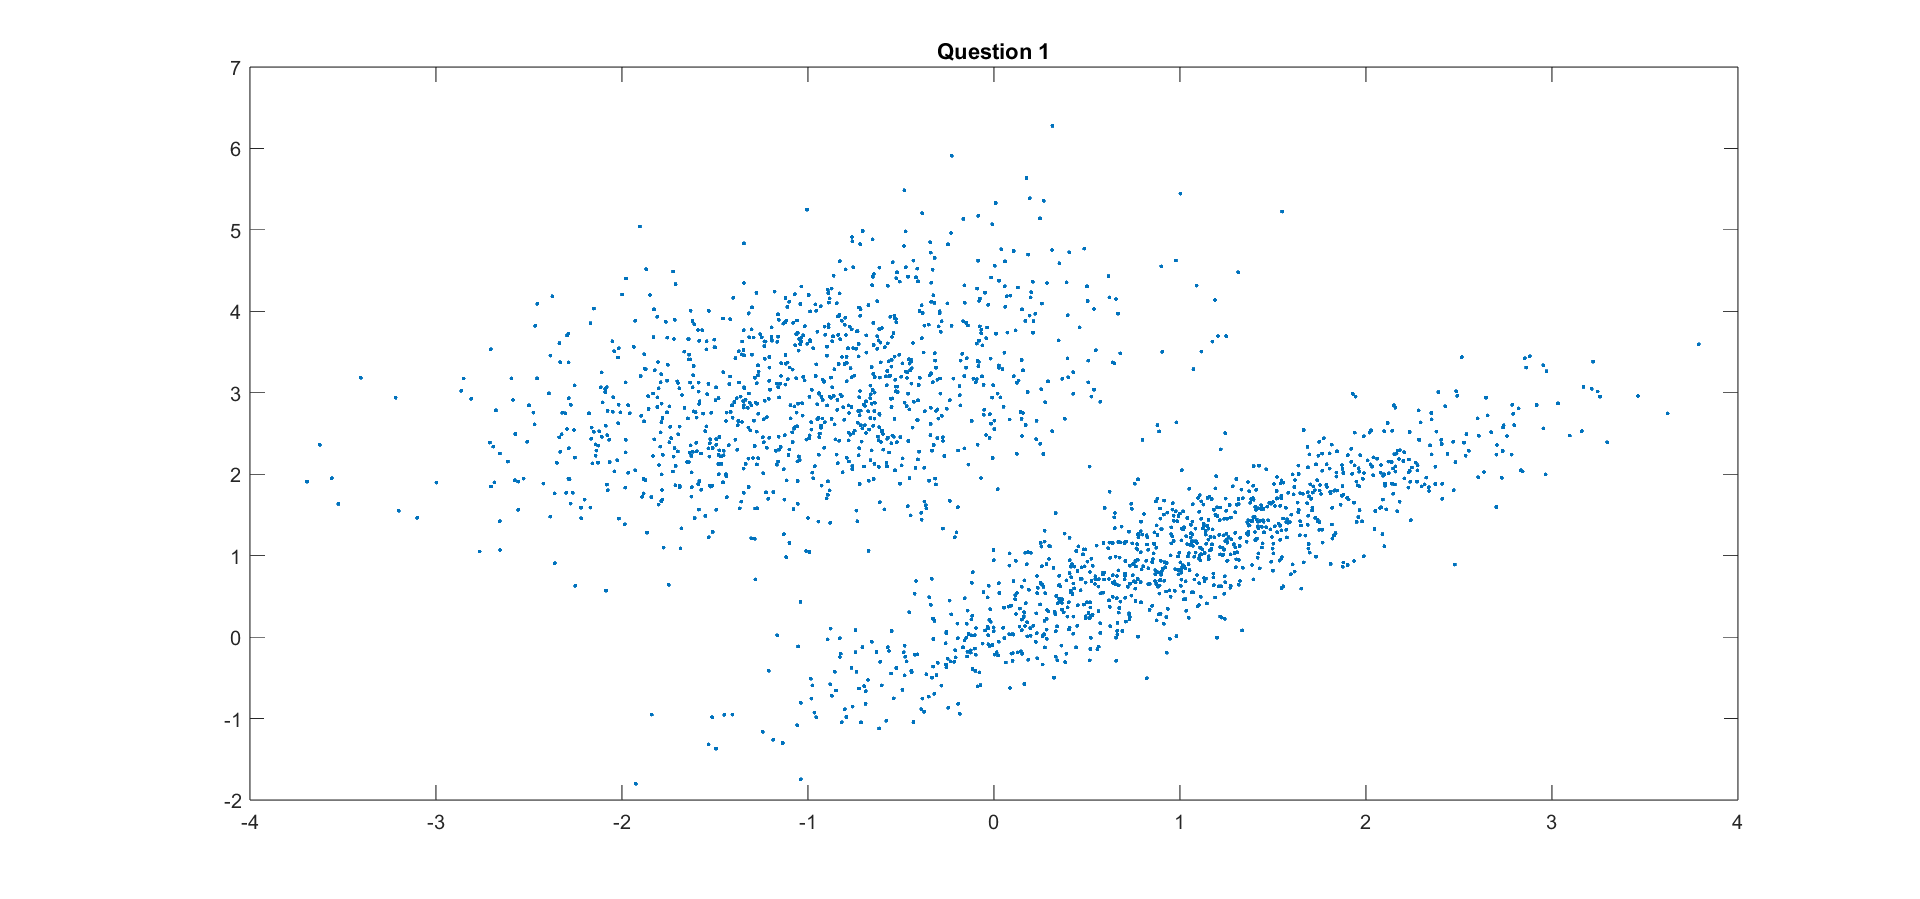
\includegraphics[width = 15cm]{images/Q1.png}
  \caption{Plot of the given data of two classes}
  \label{fig:Q1}
\end{figure}

As illustrated in Figure \ref{fig:Q1}, the dataset comprises two distinct classes that can be separated by a straight line. However, since the separating line is neither horizontal nor vertical, it is evident that a single feature alone is insufficient to achieve this separation. Consequently, both coordinates are required to effectively distinguish between the two classes.

\textbf{\emph{Question 2.}}
% Does multiple thresholding give a successful classification of the three classes?
% Explain why or why not
Multiple thresholds values were tried, where the best preformance were obtained with two threshold values at 92 and 137 as illustrated in the histogram in figure \ref{fig:Q2_hist}. The classification successfully classify the background, but fails to classify the ring against the hand, see figure \ref{fig:Q2_im}. This will be due to the similiar color of the objects and as viewed in the histogram,  there is no siginiciant distingt threshold between the regions, there exist some fluctiantions inbetween. 

\begin{figure}[h!]
  \begin{subfigure}[b]{0.5\textwidth}
       \centering
       \includegraphics[width=0.9\linewidth]{images/Q2_png.png}
       \caption{Histogram of the black and white image.}
       \label{fig:Q2_hist}
   \end{subfigure}
   \hfill
   \begin{subfigure}[b]{0.5\textwidth}
       \centering
       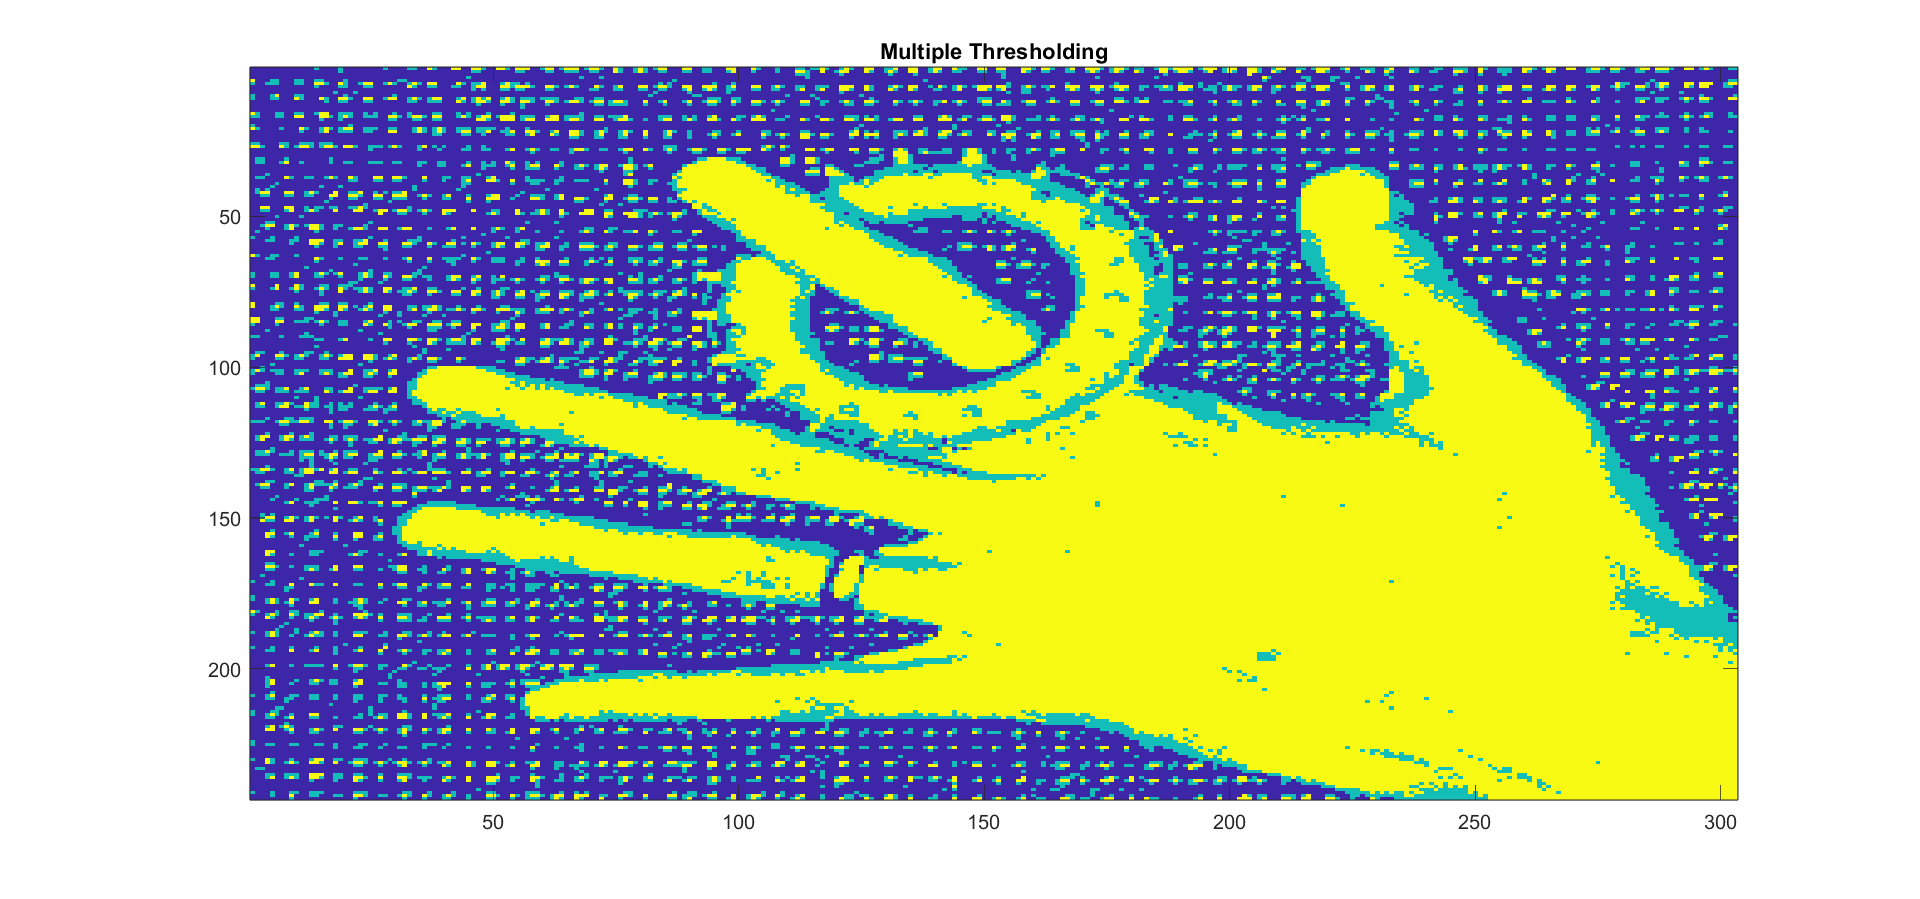
\includegraphics[width=0.9\linewidth]{images/Q2.png}
       \caption{threshold classiciation of the grayscale image}
       \label{fig:Q2_im}
   \end{subfigure}
      \caption{Mulitple thresholding and its corresponding result of an grayscale image.}
      \label{fig:Q2}
\end{figure}


\textbf{\emph{Question 3.}}
% MATLAB’s classify function uses Linear Discriminant Analysis (LDA) as default.
% What assumptions are made on the data by an LDA classifier? 
% Also, what makes a classifier linear?
Linear Discriminant Analysis (LDA) is a classification technique that operates under the assumption that the features within each class are drawn from a Gaussian (normal) distribution and that all classes share a common covariance matrix. This shared covariance matrix ensures that the decision boundaries between classes are linear, which is a defining characteristic of the classifier. Specifically, the decision boundary is represented as a linear function of the input features, making LDA particularly effective for problems where this assumption holds true.

\textbf{\emph{Question 4.}}
% Have the results improved using classification compared to thresholding? Is the classification more successful in the case with the grayscale image or single bands? Explain.
% Does it improve the classification to incorporate pairs of bands or the full RGB information? Discuss. 
% Show your results from grayscale classification, one pair of features and full RGB classification
The background more distingt distinguished when using classification and a slighter better classification of the objects, but still not successful

When comparing the preformance of mulitple thresholding and classification of the grayscle image
\section{Classification of multispectral data}
\textbf{\emph{Question 5.}}

\textbf{\emph{Question 6.}}

\section{Texture-based Classification}
\textbf{\emph{Question 7.}}



\end{document}
